\documentclass{article}
\usepackage[utf8]{inputenc}
\usepackage[spanish]{babel}
\usepackage{listings}
\usepackage{graphicx}
\graphicspath{ {images/} }
\usepackage{cite}

\begin{document}

\begin{titlepage}
    \begin{center}
        \vspace*{1cm}
            
        \Huge
        \textbf{Implementación y Diseño}
            
        \vspace{0.5cm}
        \LARGE
        StonerIt (Proyecto Final)
            
        \vspace{1.5cm}
            
        \textbf{Nelson Fernando Parra Guardia}
            
        \vfill
            
        \vspace{0.8cm}
            
        \Large
        Despartamento de Ingeniería Electrónica y Telecomunicaciones\\
        Universidad de Antioquia\\
        Medellín\\
        Octubre de 2021
            
    \end{center}
\end{titlepage}

\newpage
\section{Diseño}
Para el proyecto final, inicialmente se plantean 5 niveles: dos de los cuales tendrán enemigos normales (pequeños y múltiples) y tres de ellos serán jefes. De igual manera, se postulan los siguientes mapas, donde el bloque A será el borde de la ventana (que todos los mapas tendrán) y el bloque B, uno indestructible que le impedirá movimiento y ataques al jugador. Los mapas de las figuras 2 y 3, pertenecerán a los niveles 1 y 3 en los cuales hay que luchar con enemigos normales (explicados anteriormente) y los niveles que contengan un jefe, se van a desenvolver en un mapa abierto sin obstáculos.

\begin{figure}[h]
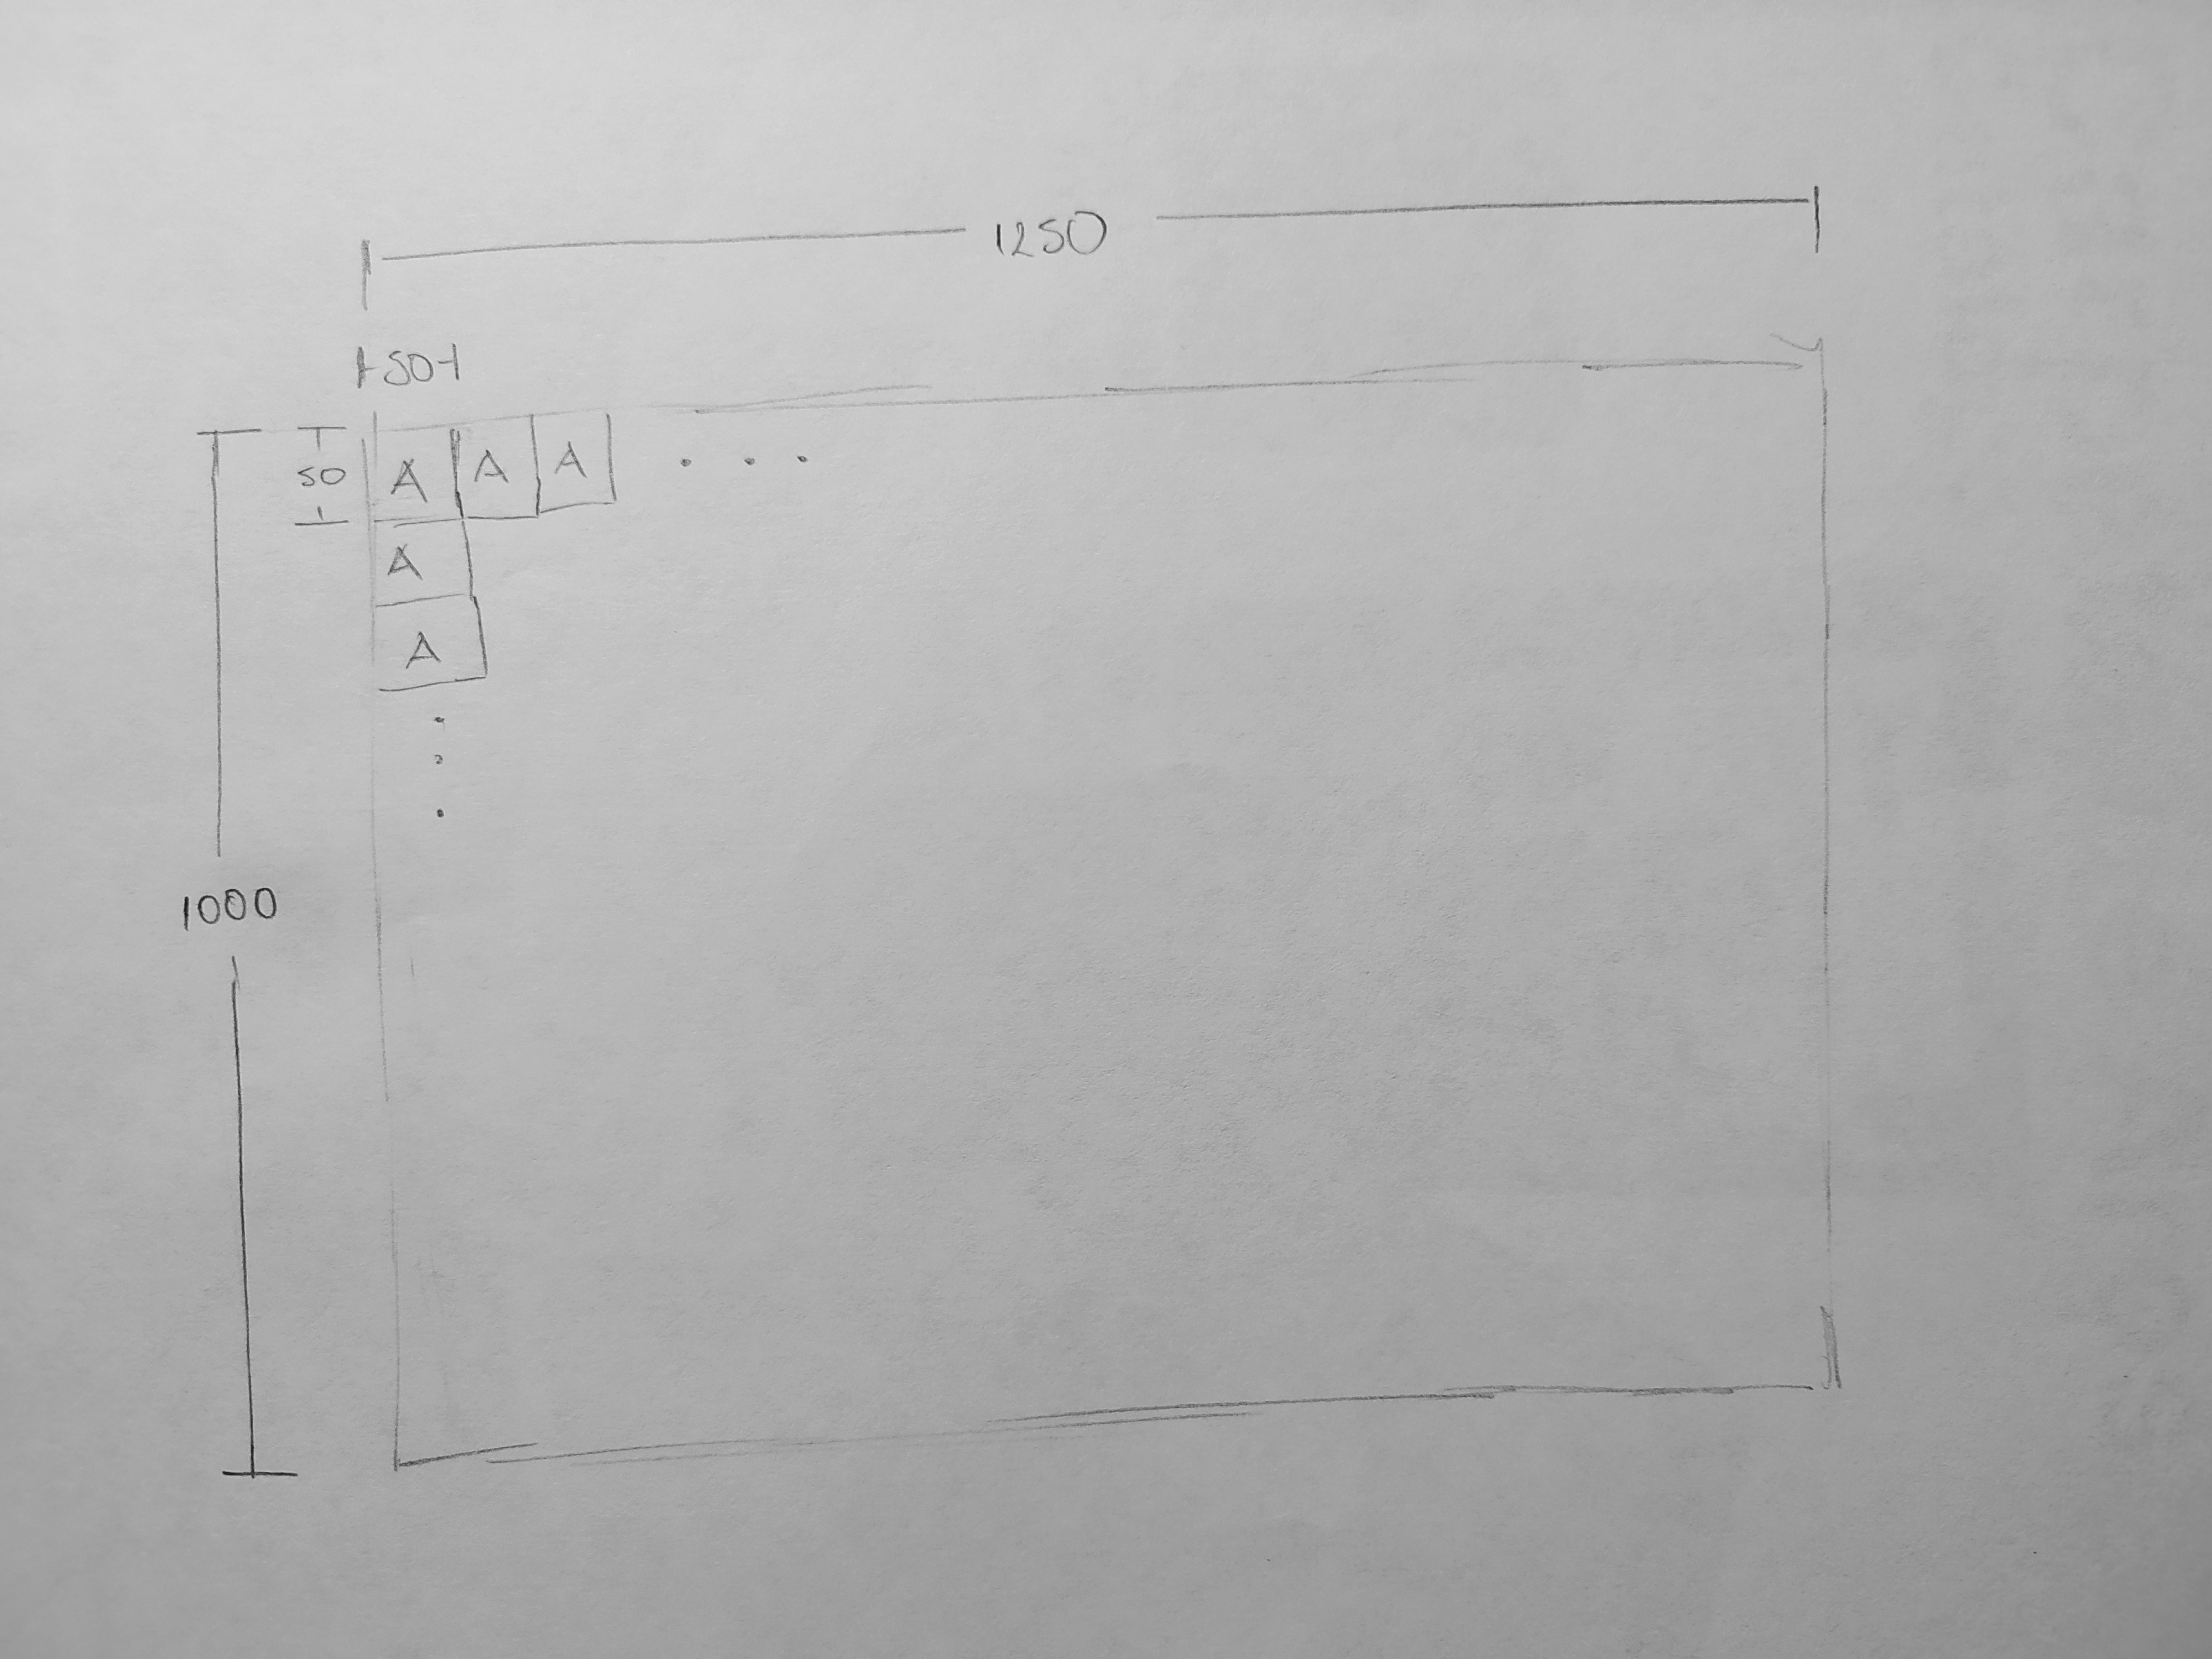
\includegraphics[width=10cm, height=5cm]{imagenes/bordes.jpg}
\centering
\caption{Contorno de los mapas.}
\label{fig:diagram}
\end{figure}

\begin{figure}[h]
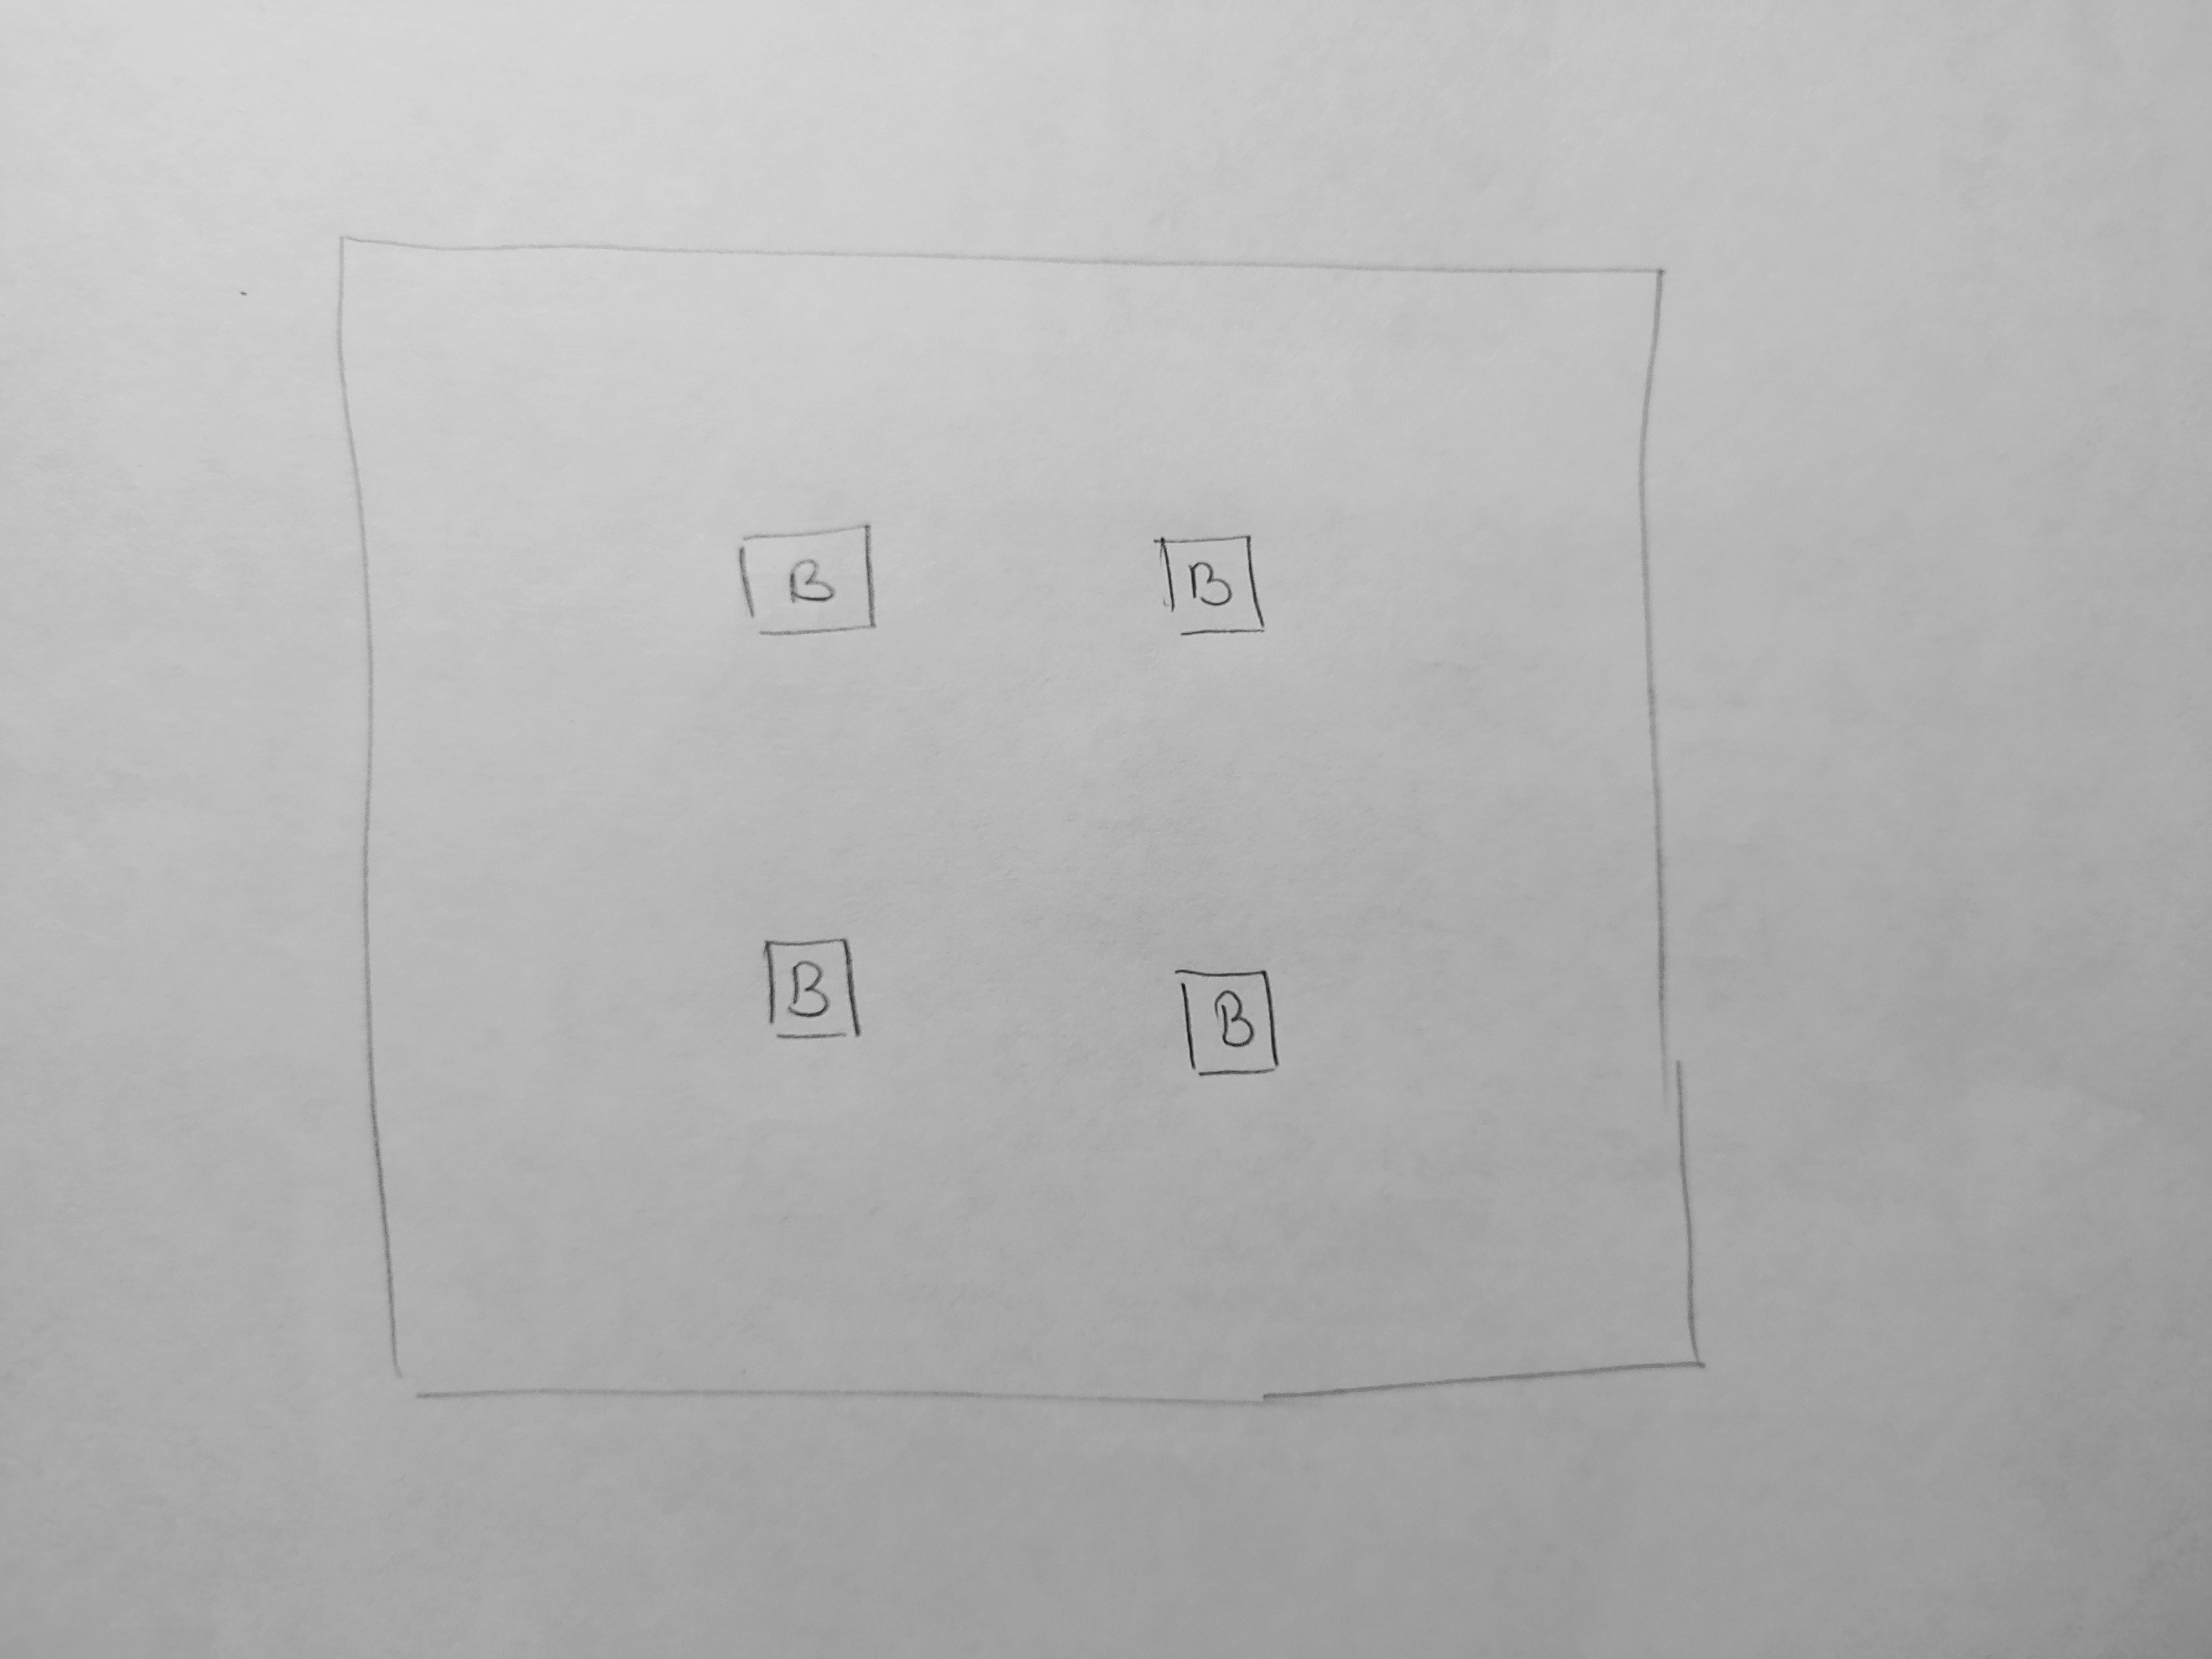
\includegraphics[width=10cm, height=5cm]{imagenes/mapa1.jpg}
\centering
\caption{Mapa nivel 1.}
\label{fig:diagram}
\end{figure}

\begin{figure}[h]
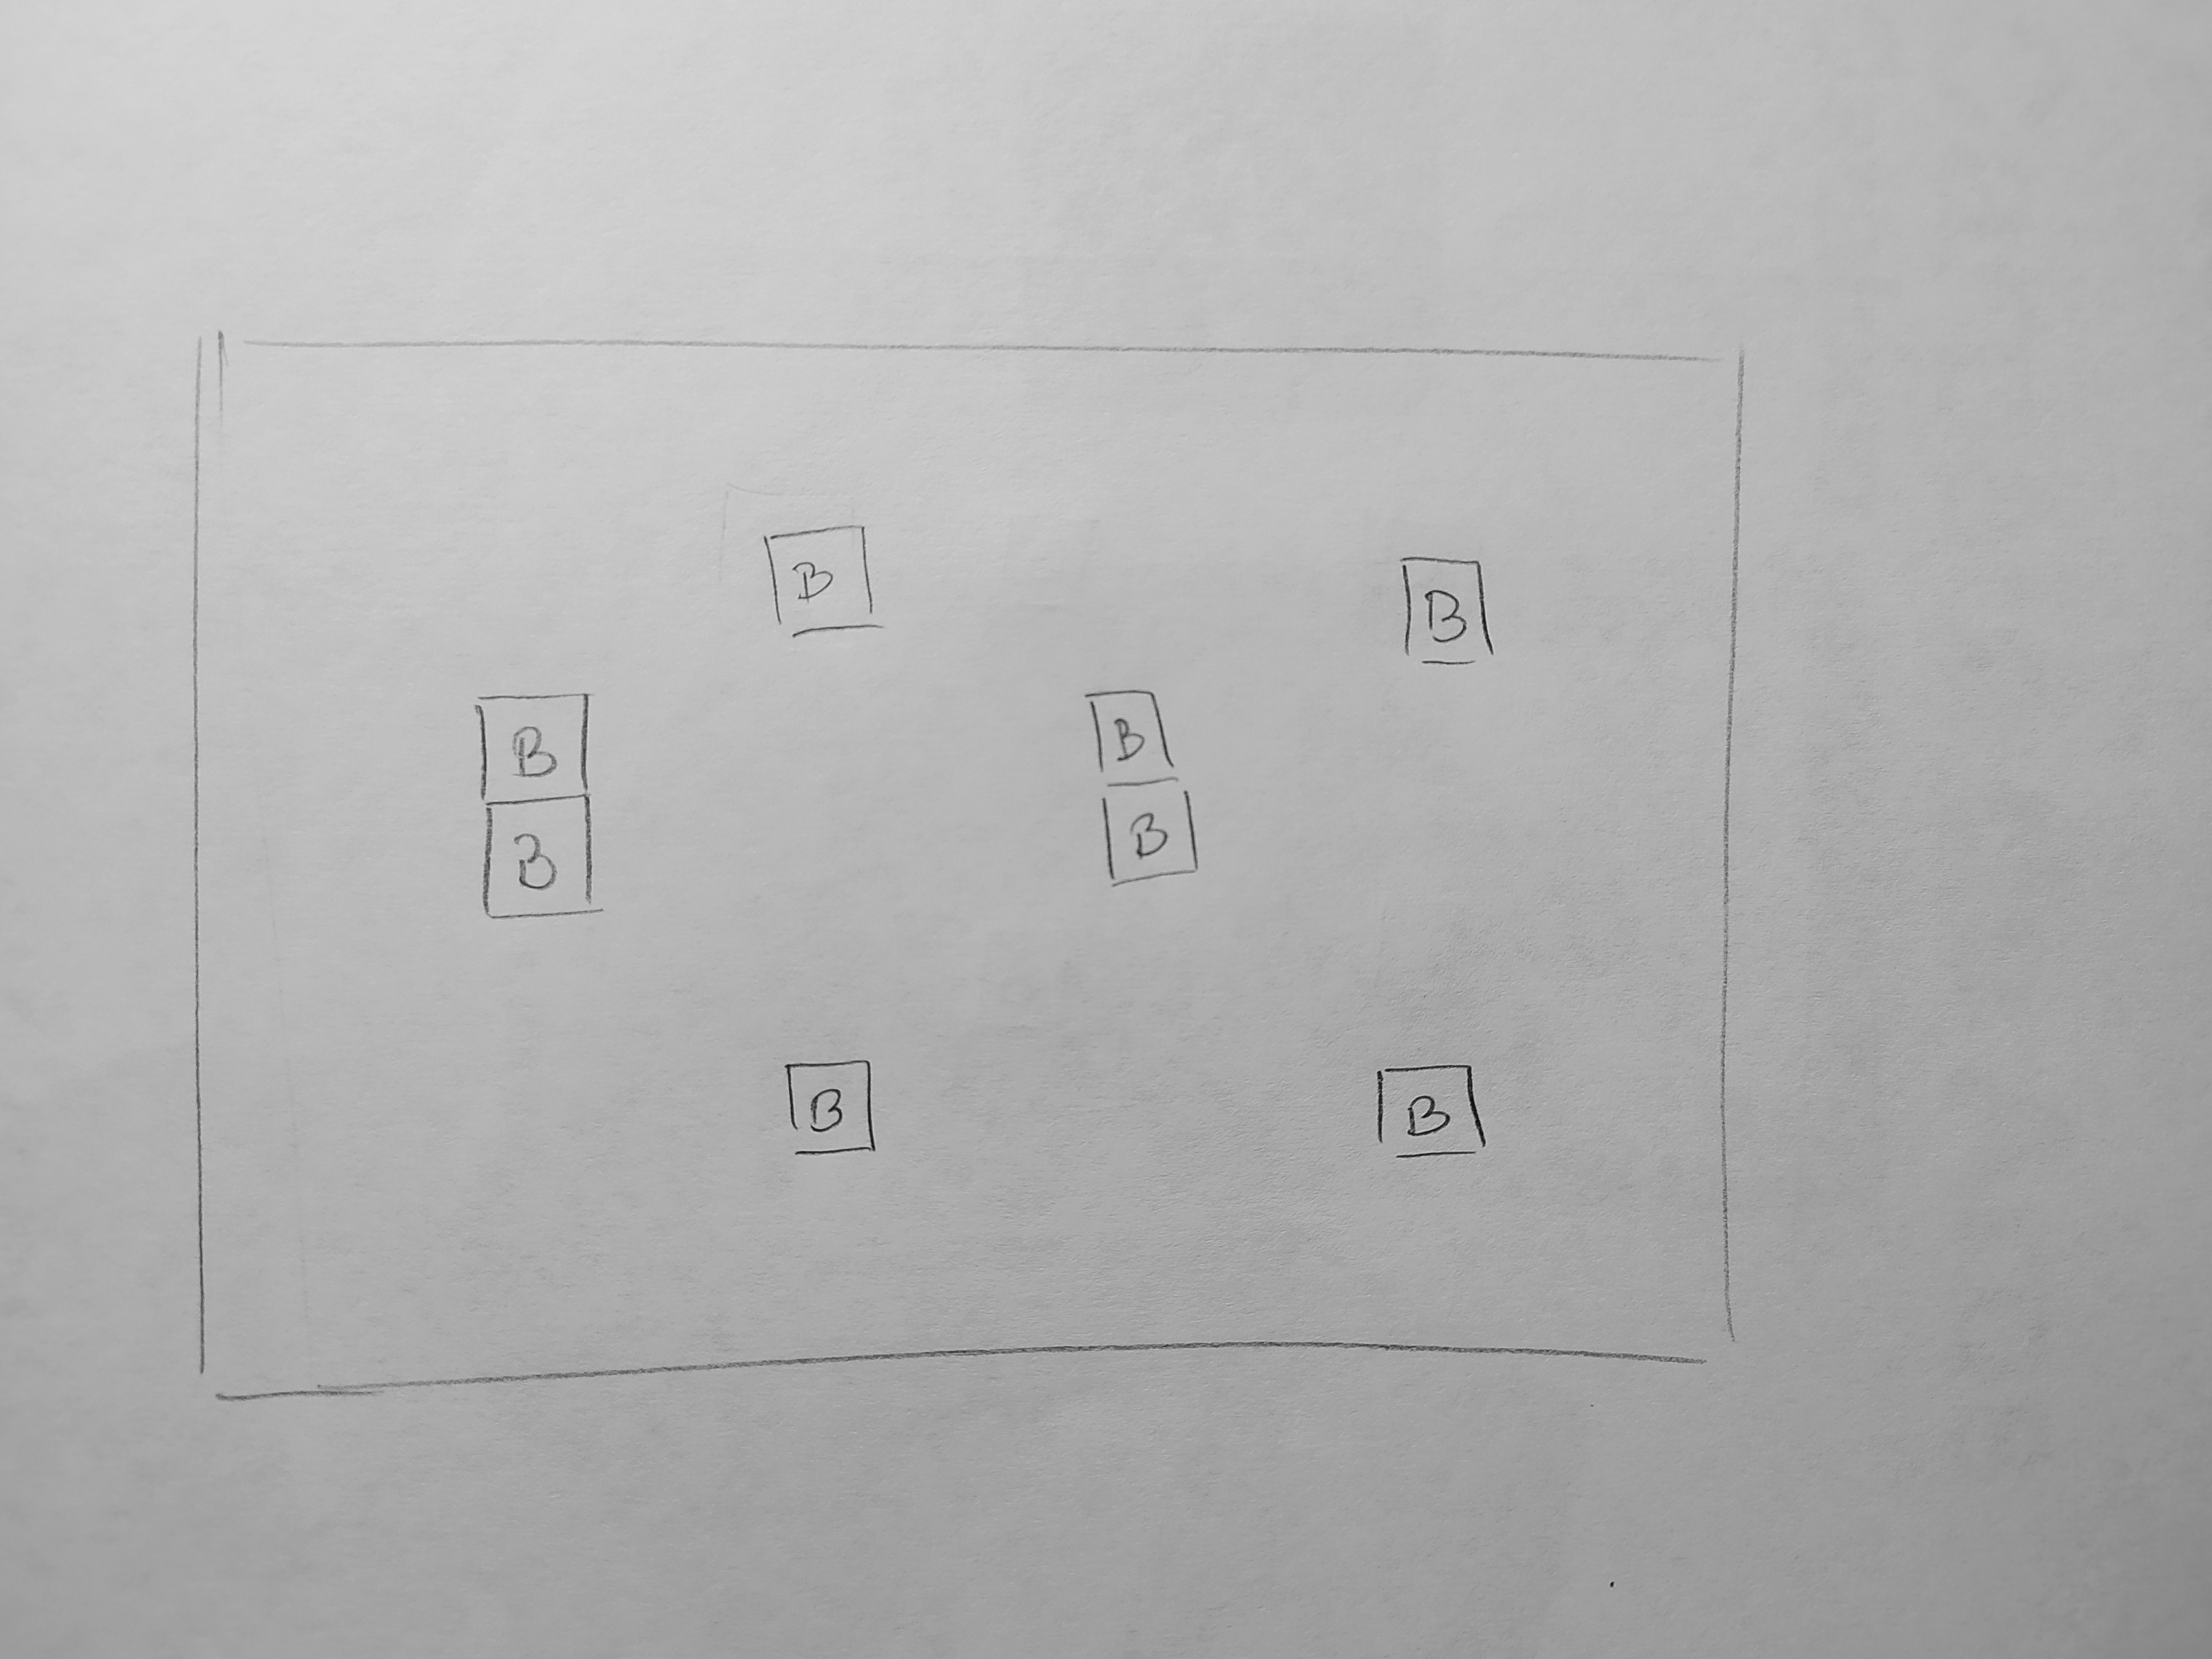
\includegraphics[width=10cm, height=5cm]{imagenes/mapa3.jpg}
\centering
\caption{Mapa nivel 3.}
\label{fig:diagram}
\end{figure}

\section{Inconvenientes}
De primeras, uno de los impedimentos que se me presenta es el hecho de colocar niveles y múltiples escenas a una misma ventana. Sin embargo, sin pensarlo mucho, se plantea que cada vez que una escena termine su función (menú o juego) todos los items de la escena se eliminan y se crean unos nuevos con la utilidad siguiente.

\end{document}
